% Apex - feature review deck (Beamer, 16:9, pdflatex)
% Build:  cd docs/slides && pdflatex apex-features.tex && pdflatex apex-features.tex
\documentclass[aspectratio=169,10pt]{beamer}

\usepackage[T1]{fontenc}
\usepackage[utf8]{inputenc}
\usepackage{textcomp}
\usepackage{helvet}
\renewcommand{\familydefault}{\sfdefault}
\usepackage{graphicx}
\usepackage{xcolor}
\usepackage{booktabs}
\usepackage{array}
\newcolumntype{L}[1]{>{\raggedright\arraybackslash}p{#1}}
\usepackage{tikz}
\usepackage{microtype}
\usetikzlibrary{positioning,arrows.meta,fit,backgrounds}

% ---- IBM Carbon-derived palette (the app's own colour semantics) ----------
\definecolor{cblue}{HTML}{0F62FE}
\definecolor{cink}{HTML}{161616}
\definecolor{cgray}{HTML}{525252}
\definecolor{cline}{HTML}{C6C6C6}
\definecolor{cpurple}{HTML}{8A3FFC}
\definecolor{cgreen}{HTML}{24A148}
\definecolor{cred}{HTML}{DA1E28}
\definecolor{cwash}{HTML}{F4F4F4}

\usetheme{default}
\usecolortheme{default}
\setbeamertemplate{navigation symbols}{}
\setbeamercolor{normal text}{fg=cink}
\setbeamercolor{structure}{fg=cblue}
\setbeamercolor{frametitle}{fg=cink}
\setbeamerfont{frametitle}{series=\bfseries,size=\large}
\setbeamerfont{framesubtitle}{size=\footnotesize}
\setbeamercolor{framesubtitle}{fg=cgray}
\setbeamertemplate{frametitle}{%
  \vspace{6pt}%
  \usebeamerfont{frametitle}\usebeamercolor[fg]{frametitle}\insertframetitle\par
  \ifx\insertframesubtitle\@empty\else
    \vspace{1pt}\usebeamerfont{framesubtitle}\usebeamercolor[fg]{framesubtitle}\insertframesubtitle\par
  \fi
  \vspace{2pt}{\color{cblue}\rule{\textwidth}{1.1pt}}\par\vspace{-2pt}}
\setbeamertemplate{itemize item}{\color{cblue}\rule[0.35ex]{0.45em}{0.45em}}
\setbeamertemplate{itemize subitem}{\color{cgray}\rule[0.35ex]{0.35em}{0.35em}}
\setbeamertemplate{footline}{%
  \hbox{\begin{beamercolorbox}[wd=\paperwidth,ht=2.4ex,dp=1.4ex,leftskip=1.2em,rightskip=1.2em]{}%
  \tiny\color{cgray}Apex --- Desktop Telemetry \& AI Driver Coaching\hfill\insertframenumber\end{beamercolorbox}}}
\setlength{\parskip}{2pt}

% ---- helpers -------------------------------------------------------------
\newcommand{\shotmax}{0.655\textheight}
\newcommand{\shot}[1]{%
  \begin{center}%
  \setlength{\fboxsep}{0pt}\setlength{\fboxrule}{0.6pt}%
  {\color{cline}\fbox{\includegraphics[width=\linewidth,height=\shotmax,keepaspectratio]{figures/#1}}}%
  \end{center}}
\newcommand{\shotw}[2]{%
  \begin{center}%
  \setlength{\fboxsep}{0pt}\setlength{\fboxrule}{0.6pt}%
  {\color{cline}\fbox{\includegraphics[width=#2\linewidth]{figures/#1}}}%
  \end{center}}
\newcommand{\shotc}[2]{%
  \shot{#1}\vspace{-2pt}{\footnotesize\color{cgray}#2\par}}
\newcommand{\kw}[1]{\textcolor{cblue}{\textbf{#1}}}
\newcommand{\code}[1]{{\ttfamily\small #1}}

\title{Apex}
\subtitle{Desktop Telemetry \& AI Driver Coaching --- Feature Review}
\author{Dany}
\institute{University of Bristol MSc $\times$ IBM --- F1 Telemetry \& Driver Coaching}
\date{18 August 2026}

\begin{document}

% ==========================================================================
\begin{frame}[plain]
  \vspace{1.2em}
  {\color{cblue}\rule{\textwidth}{3pt}}\par\vspace{1.0em}
  {\Huge\bfseries Apex}\par\vspace{0.4em}
  {\large Desktop Telemetry \& AI Driver Coaching}\par\vspace{0.2em}
  {\large\color{cgray} Feature review for supervisor meeting}\par\vspace{1.6em}
  {\small\color{cgray}
   University of Bristol MSc $\times$ IBM --- F1 Telemetry \& Driver Coaching project\par
   \vspace{0.4em}
   TORCS 1.3.9 \quad\textbullet\quad PySide6 / Qt~6 \quad\textbullet\quad IBM Granite 4.1 (local)\par}
  \vspace{1.2em}
  {\small\color{cink} Dany\par}
  {\small\color{cgray} 18 August 2026\par}
  \vspace{0.6em}{\color{cline}\rule{\textwidth}{0.8pt}}
\end{frame}

% ==========================================================================
\begin{frame}{What Apex is}{One desktop application covering the whole loop: drive, record, analyse, explain}
  \begin{columns}[T]
  \begin{column}{0.52\textwidth}
    \begin{itemize}
      \item A \kw{native desktop app} (PySide6/Qt~6 + PyQtGraph), running on
            macOS, Linux and Windows from one code base.
      \item It is the \kw{participant-facing launcher} for the driving study:
            no terminal, no CSV handling, no simulator configuration.
      \item \kw{IBM Granite 4.1} runs locally as a race engineer. It reads
            telemetry evidence and returns advice --- it never controls the car.
      \item Every model claim is \kw{checked against the telemetry} before it is
            allowed on screen, and the whole exchange is written to an audit record.
    \end{itemize}
  \end{column}
  \begin{column}{0.44\textwidth}
    \vspace{0.4em}
    \setlength{\fboxsep}{9pt}
    {\color{cwash}\fbox{\parbox{0.86\textwidth}{\color{cink}\small
      \textbf{Design rule}\par\vspace{4pt}
      \color{cgray}The application never computes telemetry truth. It renders
      what \code{f1coach-core} returns.\par\vspace{6pt}
      \color{cink}\textbf{Safety rule}\par\vspace{4pt}
      \color{cgray}The advisory model is not in the control loop. Deterministic
      code keeps control of the car at all times.}}}
    \par\vspace{0.8em}
    {\footnotesize\color{cgray}364 automated tests passing \textbullet{} lint clean}
  \end{column}
  \end{columns}
\end{frame}

% ==========================================================================
\begin{frame}{System architecture}{One process for the UI and the analysis core; the model sits beside the loop, never inside it}
  \centering
  \vspace{-2pt}
  \resizebox{\textwidth}{!}{%
  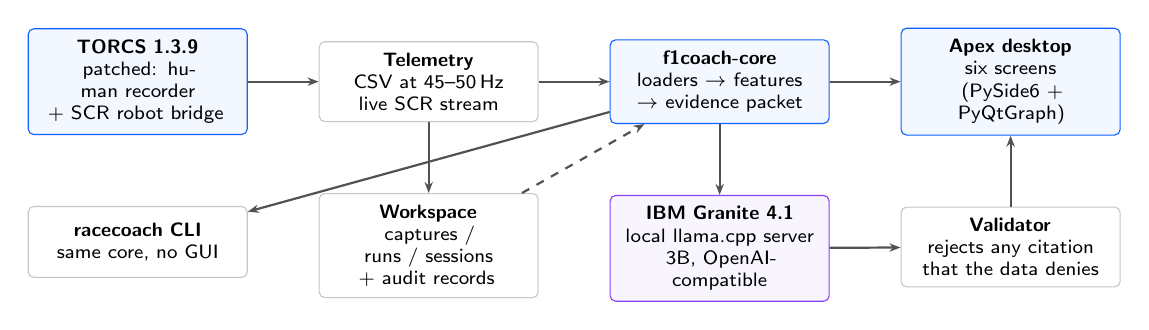
\begin{tikzpicture}[
      font=\scriptsize,
      box/.style={draw=cline,fill=white,rounded corners=2pt,align=center,
                  minimum height=9mm,inner sep=4pt,text width=25mm},
      accent/.style={box,draw=cblue,fill=cblue!5},
      model/.style={box,draw=cpurple,fill=cpurple!5},
      lbl/.style={font=\tiny\itshape,color=cgray},
      ar/.style={-{Stealth[length=4pt]},draw=cgray,thick}]

    \node[accent] (torcs) {\textbf{TORCS 1.3.9}\\\scriptsize patched: human recorder\\+ SCR robot bridge};
    \node[box,right=9mm of torcs] (csv) {\textbf{Telemetry}\\\scriptsize CSV at 45--50\,Hz\\live SCR stream};
    \node[accent,right=9mm of csv] (core) {\textbf{f1coach-core}\\\scriptsize loaders $\rightarrow$ features\\$\rightarrow$ evidence packet};
    \node[accent,right=9mm of core] (ui) {\textbf{Apex desktop}\\\scriptsize six screens\\(PySide6 + PyQtGraph)};

    \node[model,below=9mm of core] (granite) {\textbf{IBM Granite 4.1}\\\scriptsize local llama.cpp server\\3B, OpenAI-compatible};
    \node[box,below=9mm of ui] (val) {\textbf{Validator}\\\scriptsize rejects any citation\\that the data denies};
    \node[box,below=9mm of csv] (store) {\textbf{Workspace}\\\scriptsize captures / runs / sessions\\+ audit records};
    \node[box,below=9mm of torcs] (cli) {\textbf{racecoach CLI}\\\scriptsize same core, no GUI};

    \draw[ar] (torcs) -- (csv);
    \draw[ar] (csv) -- (core);
    \draw[ar] (core) -- (ui);
    \draw[ar] (core) -- (granite);
    \draw[ar] (granite) -- (val);
    \draw[ar] (val) -- (ui);
    \draw[ar] (csv) -- (store);
    \draw[ar] (core) -- (cli);
    \draw[ar,dashed] (store) -- (core);
  \end{tikzpicture}}
  \par\vspace{4pt}
  {\footnotesize\color{cgray}The dashed path is re-analysis: a stored run is reloaded
  and re-examined without touching the simulator.}
\end{frame}

% ==========================================================================
\begin{frame}{The six screens}{Everything below is a live screenshot of the current build}
  \small
  \begin{tabular}{@{}L{25mm}L{42mm}L{55mm}@{}}
    \toprule
    \textbf{Screen} & \textbf{Who uses it} & \textbf{What it does} \\
    \midrule
    Garage        & Everyone      & Session library, lap table, import and watched folders \\
    Collect Data  & Participant   & Guided three-step capture; opens the assigned TORCS race \\
    Robot Pilot   & Facilitator   & Unattended synthetic reference batches (pipeline testing) \\
    Lap Analysis  & Everyone      & Traces, corner table, driver debrief, Granite race engineer \\
    Compare       & Everyone      & Two laps on a shared distance axis with cumulative delta \\
    Live Pit Wall & Operator      & Live telemetry, tyre state and validated Granite advice \\
    \bottomrule
  \end{tabular}
  \par\vspace{0.9em}
  {\footnotesize\color{cgray}Robot Pilot is hidden unless \code{APEX\_RESEARCH\_MODE=1};
  participants never see it.}
\end{frame}

% ==========================================================================
\begin{frame}{Garage --- the session library}
  \shot{01-garage.png}
  \vspace{-1pt}
  {\scriptsize\color{cgray}First run opens a bundled sample session --- no credentials, no network.
  Purple marks the session best; deltas are measured against it. Telemetry arrives by button,
  drag-and-drop or a watched folder.}
\end{frame}

% ==========================================================================
\begin{frame}{Collect Data --- prepare}{Pseudonymous identity, a frozen study preset, and an explicit simulator check}
  \begin{columns}[T]
  \begin{column}{0.6\textwidth}
    \shot{02-collect-prepare.png}
  \end{column}
  \begin{column}{0.38\textwidth}\footnotesize
    \begin{itemize}\itemsep3pt
      \item \kw{Pseudonymous ID only} --- the field explicitly warns against
            names and email addresses.
      \item \kw{Frozen preset} \code{apex-study-v1}: \code{g-track-1} (road),
            \code{car7-trb1}, five laps, fixed render size.
      \item \kw{Simulator check} runs before the start button is enabled, so a
            broken install is caught before a participant sits down.
      \item \kw{Readiness checklist} covers the input device, the environment
            and the phase/ID assignment.
    \end{itemize}
  \end{column}
  \end{columns}
\end{frame}

% ==========================================================================
\begin{frame}{Collect Data --- drive, then hand over}{No terminal, no CSV selection, no simulator configuration at any point}
  \shotw{03-collect-drive.png}{0.80}
  \vspace{-4pt}
  \shotw{04-collect-saved.png}{0.80}
  \vspace{-3pt}
  {\scriptsize\color{cgray}Apex opens the assigned five-lap race directly and finishes the import when
  TORCS closes. The final page ends with the two actions a participant needs --- \emph{Collect another
  session} and \emph{View my laps} --- and names the folder to send to the researchers.}
\end{frame}

% ==========================================================================
\begin{frame}{Robot Pilot --- validating the pipeline before recruitment}{Facilitator-only; synthetic runs are never presented as participant data}
  \begin{columns}[T]
  \begin{column}{0.62\textwidth}
    \shot{05-robot-pilot.png}
  \end{column}
  \begin{column}{0.36\textwidth}\footnotesize
    \begin{itemize}\itemsep3pt
      \item Runs a \kw{pinned built-in robot} (\code{berniw} index 9) on the same
            track and car, three laps per session.
      \item 1--20 sequential unattended sessions; each is validated and imported
            exactly like a human capture.
      \item Stored separately under \code{captures/synthetic/} with
            \code{synthetic-robot} provenance and \code{SIM-BERNIW9-NNN} ids.
      \item The banner states the limit plainly: these runs test the collection
            pipeline; they cannot show that coaching changes human behaviour.
    \end{itemize}
  \end{column}
  \end{columns}
\end{frame}

% ==========================================================================
\begin{frame}{Lap Analysis --- the AI race engineer}
  \shot{06-analysis-granite.png}
  \vspace{-1pt}
  {\scriptsize\color{cgray}Sector ribbon, synced speed/throttle/brake strips on one distance axis,
  and a corner table with deterministic technique flags. The card is a real response from the local
  Granite 4.1: focus, action, confidence and a clickable citation --- ``show'' zooms to the cited stretch.}
\end{frame}

% ==========================================================================
\begin{frame}{How a model claim earns its place on screen}{The interesting engineering is what happens between the model and the display}
  \begin{columns}[T]
  \begin{column}{0.5\textwidth}\footnotesize
    \begin{enumerate}\itemsep4pt
      \item \code{f1coach-core} computes an \kw{evidence packet} from the lap:
            corner spans, brake points, minimum and exit speeds, coasting,
            pedal overlap.
      \item Granite receives \kw{only that packet} and must answer in a fixed
            JSON schema: issue, evidence, cause, action, confidence.
      \item A Python \kw{validator} recomputes every citation. If a corner,
            value, unit or distance span does not match, the finding is rejected
            rather than displayed.
      \item The accepted report, the prompt and the raw response are written to
            a \kw{coaching audit record}.
      \item Re-opening the same lap and reference \kw{restores} that report ---
            after revalidating the saved evidence again.
    \end{enumerate}
  \end{column}
  \begin{column}{0.46\textwidth}
    \vspace{0.2em}
    \setlength{\fboxsep}{9pt}
    {\color{cwash}\fbox{\parbox{0.88\textwidth}{\footnotesize\color{cink}
      \textbf{Why it matters}\par\vspace{5pt}\color{cgray}
      The model is treated as an untrusted narrator of numbers that the
      application already knows. A hallucinated corner or a wrong unit cannot
      reach the driver, and every claim that does reach them can be traced back
      to the exact samples behind it.\par\vspace{7pt}\color{cink}
      \textbf{Current contract}\par\vspace{4pt}\color{cgray}
      \code{ibm-granite/granite-4.1-3b}\par
      post-lap prompt \code{coach-v4}\par
      live prompt \code{granite-torcs-live-v1}}}}
  \end{column}
  \end{columns}
\end{frame}

% ==========================================================================
\begin{frame}{Driver debrief --- where the time actually went}
  \shot{07-analysis-debrief.png}
  \vspace{-1pt}
  {\scriptsize\color{cgray}Computed deterministically, with or without a model. A reference lap adds
  the debrief (``5.32\,s off your best lap; 3.86\,s of it went at T4, T1, T5''), a delta column and the
  reference trace in purple. Each point pairs a measured time loss with the largest measured difference
  over the same stretch --- and stops short of claiming the second caused the first.}
\end{frame}

% ==========================================================================
\begin{frame}{Replay --- the same stretch, on the track}{Opens beside the traces so a driver can watch and read at once}
  \begin{columns}[T]
  \begin{column}{0.44\textwidth}
    \shot{08-replay.png}
  \end{column}
  \begin{column}{0.54\textwidth}\small
    \begin{itemize}\itemsep3pt
      \item Double-clicking a debrief point replays that stretch in a separate,
            non-modal window.
      \item The line is drawn from \kw{recorded world position}; the highlighted
            segment is the stretch under discussion and the marker is the cursor.
      \item The readout follows the cursor: elapsed time, speed, throttle, brake
            and gear.
      \item A lap recorded without world position degrades to the distance-based
            view instead of drawing a broken map.
    \end{itemize}
    \vspace{0.4em}
    {\footnotesize\color{cgray}Shown here on a real captured drive, which is the data
    that carries world position. The bundled demo fixture does not.}
  \end{column}
  \end{columns}
\end{frame}

% ==========================================================================
\begin{frame}{Compare --- two laps, one distance axis}
  \shot{09-compare.png}
  \vspace{-1pt}
  {\scriptsize\color{cgray}Also the before/after view for the coaching evaluation. Speed traces overlaid
  with the cumulative time delta underneath: the slope shows \emph{where} the gap opens, not merely that it
  exists. The footer separates what changed from what is still on the table, corner by corner.}
\end{frame}

% ==========================================================================
\begin{frame}{Live Pit Wall --- advice while the car is running}
  \shot{10-live-pit-wall.png}
  \vspace{-1pt}
  {\scriptsize\color{cgray}Bridge health, tyre state and a real Granite 4.1 response with its measured
  latency. Advice is asynchronous and latest-only: a slow model delays advice, never the car. Stale advice
  is labelled rather than silently shown, and the evidence box lists the values it may rest on.}
\end{frame}

% ==========================================================================
\begin{frame}{Audit --- the record behind every answer}{Prompt, raw response, evidence packet and outcome, in one file per run}
  \begin{columns}[T]
  \begin{column}{0.56\textwidth}
    \shot{11-audit.png}
  \end{column}
  \begin{column}{0.42\textwidth}\small
    \begin{itemize}\itemsep3pt
      \item Written for \kw{every} attempt, including failures --- the record above
            names the provider, the model, the prompt version and the outcome.
      \item Contains the full evidence packet, so a reviewer can recompute what
            the model was shown.
      \item Reachable from the analysis screen through the \code{Audit\ldots}
            button; nothing has to be reconstructed from logs.
      \item This is what makes the coaching claims examinable rather than
            merely plausible.
    \end{itemize}
  \end{column}
  \end{columns}
\end{frame}

% ==========================================================================
\begin{frame}{Research data pipeline}{Raw evidence and analysis copies are kept apart on purpose}
  \small
  \begin{tabular}{@{}L{34mm}L{40mm}L{52mm}@{}}
    \toprule
    \textbf{Location} & \textbf{Holds} & \textbf{Guarantee} \\
    \midrule
    \code{captures/human/} & Raw CSV + \code{manifest.json} &
      Participant id, phase, exact TORCS command, study preset, SHA-256 per file \\
    \code{captures/synthetic/} & Robot reference batches &
      Marked \code{synthetic-robot}; never mixed with participant data \\
    \code{runs/} & Validated copies + \code{meta.json} &
      Sample count, columns, laps seen, cadence; what analysis reads \\
    \code{sessions/} & Canonical per-lap CSV + coaching audits &
      What the Garage lists and the Analysis screen opens \\
    \bottomrule
  \end{tabular}
  \par\vspace{0.8em}
  {\footnotesize\color{cgray}
  Telemetry schema \code{apex-human-v2}: more than 100 raw or directly exposed
  TORCS channels at roughly 45--50\,Hz, including per-wheel wear, temperature,
  pressure and graining. The whole tree relocates with \code{APEX\_WORKSPACE}
  so study data can sit on an approved volume.}
\end{frame}

% ==========================================================================
\begin{frame}{The same core without a GUI}{\code{racecoach} --- for automation, recovery and reproducible checks}
  \small
  \begin{tabular}{@{}L{40mm}L{88mm}@{}}
    \toprule
    \textbf{Command} & \textbf{Purpose} \\
    \midrule
    \code{import} / \code{list} & Import a TORCS exporter CSV; list stored runs \\
    \code{analyze} & Compute metrics for a stored run \\
    \code{coach} & Post-run LLM feedback, optionally grounded in a code overview \\
    \code{run} & Drive the car and capture telemetry, with an optional live advisor \\
    \code{capture-human} & Facilitator fallback for participant capture \\
    \code{capture-synthetic} & Pinned unattended robot reference sessions \\
    \code{report} & Render the post-race HTML report \\
    \bottomrule
  \end{tabular}
  \par\vspace{0.8em}
  {\footnotesize\color{cgray}The desktop app, the CLI and the notebooks are three faces
  of one package: nothing in the UI can disagree with what the CLI computes.
  A contract-only demo needs no model download at all:
  \code{python -m racecoach.granite.smoke --mock}.}
\end{frame}

% ==========================================================================
\begin{frame}{Engineering status}{Where the build stands today}
  \begin{columns}[T]
  \begin{column}{0.48\textwidth}\small
    \textbf{Done}
    \begin{itemize}\itemsep2pt
      \item All six screens implemented and under test.
      \item Native TORCS 1.3.9 overlay: human telemetry recorder, SCR robot
            bridge, locked study preset.
      \item Local Granite 4.1 integration end to end, post-lap and live, with
            validation and audit records.
      \item Human capture, synthetic reference capture, and the full storage
            contract.
      \item Windows build and per-user installer; macOS and Linux from the same
            source.
      \item \textbf{364 automated tests passing}, lint clean.
    \end{itemize}
  \end{column}
  \begin{column}{0.48\textwidth}\small
    \textbf{Open}
    \begin{itemize}\itemsep2pt
      \item Pilot acceptance run with a real participant, end to end.
      \item Captures so far are short pilot drives; no multi-lap human dataset
            yet, so no before/after coaching result can be claimed.
      \item World position is recorded by the human capture path but not by the
            live SCR path, so the replay map is limited to captured drives.
      \item Race Engineer Q\&A panel remains a stretch goal.
      \item Report export exists; packaging it into the study protocol is next.
    \end{itemize}
  \end{column}
  \end{columns}
\end{frame}

% ==========================================================================
\begin{frame}{Next steps}{What I propose to do before the next review}
  \begin{enumerate}\itemsep6pt
    \item \kw{Run the pilot acceptance session} end to end on the Windows build,
          with a real participant and the frozen \code{apex-study-v1} preset ---
          this is the last unproven link in the chain.
    \item \kw{Collect a multi-lap baseline dataset} so that Compare can finally
          be used for what it was built for: before and after coaching.
    \item \kw{Add world position to the live SCR path} so replay works for live
          sessions as well as captured ones.
    \item \kw{Freeze a versioned study preset} after pilot evidence and
          supervisor approval, rather than continuing to develop against
          \code{apex-study-v1}.
  \end{enumerate}
  \vspace{0.8em}
  {\footnotesize\color{cgray}Question for this meeting: is the pilot protocol ready
  to be run as it stands, or should the preset change first?}
\end{frame}

% ==========================================================================
\begin{frame}{Note on the screenshots}{So the evidence in this deck is itself auditable}
  \small
  \begin{itemize}\itemsep4pt
    \item Every screenshot is the current build, rendered headless from the
          repository at commit \code{d33350d} on 18 August 2026.
    \item The coaching content on the Analysis and Live Pit Wall slides is a
          \kw{real response} from the local \code{ibm-granite/granite-4.1-3b}
          server, not a mock or a canned reply. Latency shown is measured.
    \item The Garage, Analysis, Debrief and Compare screens use the bundled
          three-lap sample session, which ships with the application.
    \item The Replay screen uses a real captured drive, because that is the data
          that carries world position.
    \item On the Collect Data and Robot Pilot slides the \kw{screens are real}
          but are shown in their completed states; running them for the
          screenshot would have required a live TORCS session and a full
          synthetic batch.
  \end{itemize}
\end{frame}

\end{document}
